\begin{figure}[H]
\centering
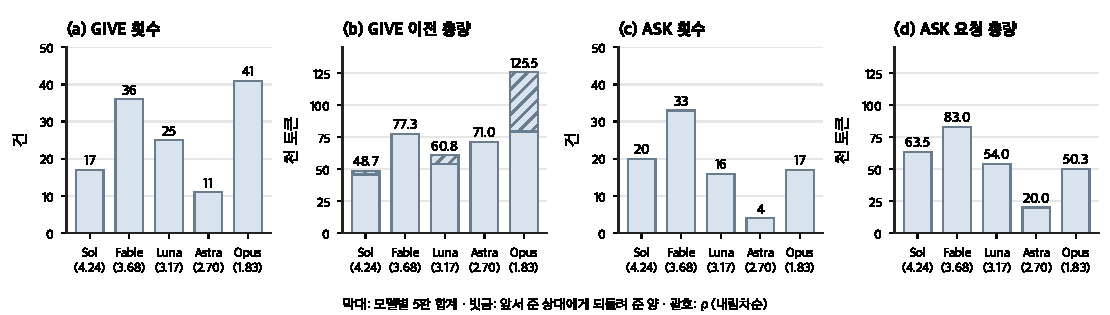
\includegraphics[width=\textwidth]{cogsci2027/ko/figures/fig_appendix0_give_ask_20261030.pdf}
\caption{\textcolor{blue}{모델별 5판의 GIVE와 ASK 총량. (a) GIVE 횟수, (b) GIVE 이전 총량, (c) ASK 횟수, (d) ASK 요청 총량이다. 모델은 $\rho$ 내림차순인 Sol, Fable, Luna, Astra, Opus로 배열했다. 막대는 5판의 합계이고 회색 점은 0을 포함한 각 판의 값이다. 총량의 단위는 천 토큰이다. 횟수는 완료된 행동 사건 수로, 한 응답의 여러 행동도 각각 센다. ASK 완료는 요청 발행을 뜻하며 이행 여부와는 구별한다. GIVE는 재이전을, ASK는 반복 요청을 포함한다. 전체 25판에서 GIVE는 130건·383,276토큰, ASK는 90건·270,800토큰이다. 행동 기회나 참여 기간으로 정규화하지 않았다.}}
\label{fig:appendix0-give-ask}
\end{figure}
